\section{Empirical Evidence}

\noindent Our empirical analysis integrates farmers' trading records, subjective market expectations, and objective measures of time-varying competition to examine the role of storage in improving smallholder welfare. Specifically, it investigates how storage enables inter-temporal arbitrage, allowing farmers to sell in more competitive farm-gate oligopsonistic markets—an aspect often overlooked in smallholder market research.

Existing observational data are insufficient, as micro-surveys typically capture post-trade information (e.g., transaction prices, storage volumes) but lack measures of temporal market competitiveness, such as buyer visits and price offer frequency after harvest. Thus, a survey-based approach is necessary to assess how storage decisions and local procurement market structures shape farmer bargaining power.

This study surveys both farmers and middlemen in a Central China county where Fuji apple cultivation dominates. Given the region's reliance on a single cash crop and the strategic role of cold storage in marketing decisions, it provides an ideal setting to analyze the interaction between storage and market competition.


%------------------------------------------------------%
\subsection{Field Site: a County in Central China}
\noindent Yanchang County, Shaanxi province, China (see Figure \ref{Figure: Yanchang}), serves as an ideal location to study farmers' marketing and storage decisions. The county is home to numerous small-scale farmers who heavily rely on a single cash crop, primarily Fuji apples, for their livelihoods. Each village within the county possesses a central market where farmers sell their produce, attracting middlemen and traders. Cold storage facilities are also available for farmers to rent or purchase, providing them with access to these inputs. In 2024, the fruit storage facilities in the entire county can accommodate up to 180,000 tons of fresh apples, with most of the capacity utilized in a given year.

\begin{figure}[thp]
\centering
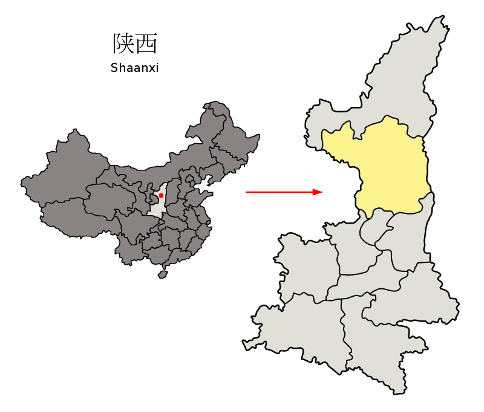
\includegraphics[width=0.6\textwidth]{Figures/yanchang_map.png}
\caption{Location of Yanchang County in China}
\label{Figure: Yanchang}
\end{figure}

The apple farmers in Yanchang County predominantly cultivate late-maturing Fuji apples, which constitute approximately 85-90\% of the production. Some farmers also grow mid-maturing apples (5-10\%) and early-maturing apples (around 5\%). Farm-gate prices range from 2.5 to 12 yuan/kg and can be checked regularly. The yield per acre does not significantly differ among the three apple varieties.

Although there are over 260 villages in the county, the average number of fruit storage facilities is slightly over 100, meaning that there is less than one facility per administrative village. Cold storage facilities owned by apple growers in Yanchang County can be classified into two types: small-scale facilities capable of storing up to 50 tons and medium-sized facilities with a capacity of up to 500 tons. According to the government report, only 1.3\% of farmers possess their own small-scale cold storage facilities. However, many farmers rent cold storage facilities established by the township and large merchants. It is worth noting that the quality of fruit storage facilities constructed by township governments is subpar compared to those built by farmers themselves. Farmers contribute 60\% of the investment, while the government subsidizes the remaining 40\%.

Farmers in Yanchang County who do not adopt cold storage facilities have to sell their harvest within a month. On the other hand, farmers using cold storage facilities need to consider various factors and market conditions, including the time-varying competition among traders. With cold storage, they can market their produce until April or May of the following year without significant deterioration. Furthermore, they are not necessarily limited to selling to middlemen but also sometimes do retail selling to consumers directly, as storage facilities grant them temporal flexibility to find more potential buyers.


%------------------------------------------------------%
\subsection{Data}
\subsubsection{Sampling Procedure}
\noindent This study employs empirical tests using data collected from two rounds of a survey of 615 smallholder apple growers in Yanchang County, Central China, covering the 2024/2025 agricultural season. With Institutional Review Board (IRB) approval, the survey was conducted between October 10, 2024, and December 13, 2024. Given that the harvest season for Fuji apples in Central China concludes in mid-to-late October, followed immediately by the lean season, this period provides a relevant timeframe to analyze the evolving market conditions faced by farmers.

The survey was conducted in collaboration with the Yanchang Women's Federation (YWF), an organization responsible for public welfare and rural development in Yanchang County. In coordination with the Yanchang County Agricultural Bureau, the YWF facilitated access to micro-level data on apple growers, enabling a structured sampling approach. A one-layer stratified random sampling method was employed based on geographical location. Yanchang County consists of one urban subdistrict and seven rural towns. To ensure representativeness, the Yanchang County Agricultural Bureau determined the approximate sampling proportion for each town based on the number and density of fruit farmers (30\%:15\%:15\%:15\%:10\%:5\%:5\%:5\%). Following these proportions, smallholder apple-growing households were randomly selected from rosters provided by administrative villages within each town.

For the purpose of this study, smallholder apple growers are defined as farmers who cultivate no more than 50 mu of land and derive at least 90\% of their agricultural income from apple production. Additionally, to maintain sufficient sample sizes across towns, a minimum of 10 participating apple growers was ensured in each town, though no minimum was imposed at the village level.

The survey targeted farmers whose primary source of income is derived from growing red Fuji apples. The interviews were conducted with the household head, except in cases where the household head was elderly and no longer part of the active labor force. In such instances, the survey was conducted with the primary labor force member of the household.



\subsubsection{Measurements of Farmers' Storage Usage and Procurement Competitiveness}
\noindent The survey examined apple growers' cold storage usage and marketing timing decisions as our key dependent variables. First, \textit{Storage-Usage-Binary} is a binary variable indicating whether a farmer used cold storage at harvest, taking a value of 1 if storage was used and 0 otherwise. Second, \textit{Storage-Usage-Type} further categorizes storage choices into four groups: \texttt{Not\_use} (no storage, corresponding to $Storage\_Usage\_Binary = 0$), and \texttt{Rent\_large}, \texttt{Rent\_small}, or \texttt{Self\_built} (all indicating some form of storage, corresponding to $Storage\_Usage\_Binary = 1$). Third, \textit{Time-to-Sell} represents the delay between harvest and sale, identically saying "the storage time". I classified sales occurring in October to a time-to-sell of 1--4 weeks post-harvest, November to 5--8 weeks, and so forth, creating interval-censored data where the exact selling time is known only within predefined intervals (1--4, 5--8, 9--12, or 13--28 weeks). 

To capture inter-temporal variations in oligopsony power among buyers, farmers were asked to report:
\begin{enumerate}
    \item The number and magnitude of price offers they received from middlemen in both October and December;
    \item Their subjective perceptions of the level of buyer competition at harvest time (ranging from 1 to 5);
    \item Their expectations regarding changes in the number of traders over the subsequent three months (i.e., from October 2024 onward).
\end{enumerate}

To assess the welfare implications for smallholder farmers, the survey collected data on their total annual agricultural income, production costs, storage costs, and other demographic characteristics.

To complement the farmer survey with market-level insights, an additional buyer survey was conducted in December 2024, targeting 15 buyers, including the top five most influential local traders. These buyers were asked to:
\begin{enumerate}
    \item Identify the specific villages they had visited during the October harvest;
    \item Report the cold storage facilities they had procured from over the past two months.
\end{enumerate}
As \cite{macchiavello2021competition} illustrated the number of mills within a 10 km radius from the mill as the baseline measure of competition, the two measures above allow for an objective assessment of the number of buyers operating in each village during the post-harvest period, providing an empirical measure of buyer concentration and inter-temporal competition.


\subsubsection{Full Sample and Sub Samples}
\noindent We have valid complete data for 549 smallholder apple-growing household observations, which would serve as our full sample. Of these, there are 


%------------------------------------------------------%
\subsection{Descriptive Statistics}
\noindent

The distribution of selling weeks by storage type is shown in Figure




\subfile{Tables/descriptive_statistics.tex}



%------------------------------------------------------%



%------------------------------------------------------%
%------------------------------------------------------%
\newpage
\subsection{Further Discussions}
\subsubsection{Time-Varying Competition Estimation}
\noindent To quantitatively evaluate the competitiveness of the oligopsonistic market faced by farmers, the study will employ an adapted version of the Lerner Index, denoted by $H$ as follows:
\begin{equation}
    H = \frac{E_t(P^w_{t+1}) - MC_t - P_t^f - S_{t,t+1}^w}{E_t(P^w_{t+1})}
\end{equation}
where $P^w_{t+1}$ captures the wholesaling price of downstream sales in month $t+1$ reported by intermediaries, $P_t^f$ represents the farm-gate price reported by farmers after the harvest in month $t$, $S_{t,t+1}^w$ shows the trader's storage cost from period $t$ to $t+1$, and $MC_t$ depicts the sum of other marginal costs of traders. In other words, the index captures the ratio of the trader's mark-up and their downstream selling price. 

The modified Lerner index could be also regarded as the pass-through of marginal product into the farm-gate price as the primary proxy for buyer's power, like in the approaches used by \cite{bergquist_dinerstein_2020} and \cite{atkin2015s}. The closer this ratio is to zero, $H \rightarrow 0$, the more competitive the oligopsonistic markets are perceived to be.

While our modified Lerner index offers a succinct measure of monopsony power, its practical application is limited due to challenges in accurately measuring traders' costs. However, since the inter-temporal behavior of prices and costs is our main focus, the delta of the Lerner Index should be reliable when we have a consistent series of traders' operational costs and storage expenses. 

To collect traders' marginal cost data and to control for demand shocks and variability, I will conduct another round of surveys on traders. The survey will include their operational costs and trading volume, and inquire about the existence of significant market events throughout the supply chain, such as fluctuations in market demand and changes in consumer preferences, natural disasters, or export/import markets.


%------------------------------------------------------%
\subsubsection{Extended Marketing Opportunities}
\noindent The adoption of cold storage has greatly extended the marketing opportunities of farmers in terms of both timing and channels. The sample of 413 households has confirmed that cold storage could greatly improve the bargaining power of farmers and boost their expected income through two primary channels:
\begin{itemize}
    \item \textbf{Better Sales Timing}: Cold storage enables farmers to store their harvest and sell at higher prices during the extended selling period. Farmers who do not use cold storage sell all their apples within one month of harvesting, while farmers who use cold storage can choose the optimal time to sell until June of the following year, allowing for a complete sales cycle lasting up to eight months. The result of my surveys shows that farm-gate prices during the first one or two months after harvest tend to be lower throughout the farming year due to the significant instantaneous supply. However, it remains unclear whether the higher farm-gate prices observed during the first post-harvest period reflect a monopsony market environment, which needs further exploration.
    
    \item \textbf{More Sales Channels}: The adoption of cold storage has expanded farmers' sales channels. It allows them to sell their harvest not only to the traders who frequently visit in late October or November and offer lower prices (ranging from 4 to 9 yuan/kg), but also to consumers through E-commerce platforms like WeChat and Taobao, where they can ask for higher prices (ranging from 10 to 14 yuan/kg). Consequently, the use of cold storage empowers apple growers to decide whether to sell in bulk or retail, depending on prevailing market conditions.
\end{itemize}


%------------------------------------------------------%
\subsubsection{Low Storage Adoption}
\noindent The adoption of cold storage among apple growers remains low. Although most of our survey respondents have the option to either rent large cold storage or build their small-scale storage, more than 85\% of them choose not to do so for the following reasons:
\begin{itemize}
    \item \textbf{Unbalanced Scale of Cold Storage}: Most of the available collective cold storage facilities are too large (over 100 tons), resulting in a low individual harvest-to-storage-volume (HSV) ratio, which leads to high costs for cold storage adoption. The storage capacity of cold storage in many villages and towns is excessively large, often hundreds or thousands of tons. To utilize cold storage, many farmers need to store their produce collectively, a decision-making process that is difficult to scale in the village, resulting in underutilized cold storage facilities. 
    
    However, I found that small cold storage units (approximately 20 to 40 tons) built by villagers have a higher utilization rate. Farmers only need to store their own harvest, without having to cooperate with others. As soon as one household in the village benefits from selling at a higher price, many other farmers follow suit, creating a positive effect. Nevertheless, due to low output, most individual apple farmers cannot fully leverage the advantages of cold storage capacity, which leads to doubts about the feasibility and cost-effectiveness of investing in cold storage.

    \item \textbf{High Transportation Loss and Cost of Usage}: When the cold storage is far from the apple orchard, transportation in the mountainous terrain becomes inconvenient, resulting in significant transportation losses. Additionally, the cost of using cold storage is relatively high. Renting either collective cold storage or storage owned by others in the village incurs storage fees ranging from 0.20 to 0.40 yuan per kilogram, regardless of the duration of storage. Considering that the price of apples per kilogram has fluctuated between 2.5 and 4.5 in recent years, the cost of using cold storage is not insignificant. In contrast, when using small self-built cold storage (with a capacity of 20 tons), the maintenance cost ranges from 250 to 350 yuan per month.
    
    Assuming a farmer's annual apple output is 10,000 kilograms, and they need to store them for 3 months to secure a higher price offer, the cost of renting cold storage would range from 2,000 to 4,000 yuan, while the maintenance fee for their storage would range from 750 to 1,050 yuan. The former is two to three times higher than the latter.

    \item \textbf{High Construction Investment}: The total cost of a self-built small cold storage with a 20-ton capacity is approximately 90,000 yuan, with government subsidies ranging from 40,000 to 50,000 yuan. However, some farmers are burdened with debts and cannot afford to invest more than 40,000 yuan in construction.

    \item \textbf{Risk Aversion}: To convert harvested fruits into profits quickly, many extreme risk-averse farmers opt to sell their produce at lower prices early in the season to reduce uncertainty, rather than relying on cold storage and future market conditions. During the harvest season in October, many fruit dealers enter rural areas to make direct purchases. Among farmers, obtaining income directly during the harvest season is often considered the most straightforward approach. It's worth noting that among the surveyed farmers, those with higher levels of education tend to delay selling apples, which aligns with cold storage ownership and risk preferences.
\end{itemize}

However, at the same time, Yanchang is still experiencing a shortage in the supply of storage facilities. Cold storage facilities across the county are consistently full each year. In other words, the overall storage capacity currently falls short of demand. Consequently, rental storage fees have increased from 0.4 yuan/kg last year to 0.5 yuan/kg this year. The inventory of large merchants' cold storage is complex, with about 50\% being the owners' own apples, and the remaining apples are mostly from small fruit merchants and farmers stored in their facilities.

In summary, the impact of cold storage adoption on farmers' welfare is closely related to the storage's "relative" capacity, i.e., the harvest-to-storage-volume (HSV) ratio. If apple production is sufficiently large to fill the entire cold storage, utilization rates are high, and farmers can choose to store their harvests with confidence, anticipating higher prices at the end of the year or even during the Spring Festival. In such cases, cold storage adoption tends to benefit farmers the most.

Conversely, when apple production is low compared to the cold storage scale, cold storage is more likely to be abandoned. Farmers believe that the profits from later sales may not cover the sunk costs, communication expenses, and losses associated with using cold storage and transporting apples. Consequently, they are more inclined to sell their produce promptly during the harvest season. However, our on-site survey indicates that farmers with access to cold storage have better bargaining power than those who do not. In this scenario, access to storage serves as a deterrent rather than being used actively, as traders often possess better storage facilities than farmers. Storage is not primarily used to preserve products but rather as a signal or implicit threat to compel traders to offer more competitive prices.

